%%%%%%%%%%%%%%%%%%%%%%%%%%%%%%%%%%%%%%%%%%%%%%%%%%%%%%%%%%%%%%%%%%%%%%%%%%%%%%%%%%%%%
% Industrial implementations of RL
%
%
% 
%%%%%%%%%%%%%%%%%%%%%%%%%%%%%%%%%%%%%%%%%%%%%%%%%%%%%%%%%%%%%%%%%%%%%%%%%%%%%%%%%%%

This chapter starts with a literature review on the most famous RL applications in history.  Applications in this section have all been widely covered by the media and are well known amongst researchers and industrial practitioners alike.  Then, a review on RL applications catered towards the process control industry will be provided. Finally, this chapter is concluded with an impressive application of RL for power optimization. The main contribution of this chapter is the conducted literature view.

\section{Renowned triumphs}
The world witnessed, for the first time, artificial intelligence learning and playing games with a mere camera placed in front of the computer screen \cite{dqn1, dqn2}!  In this application, a general RL agent \textit{successfully} conquered various ATARI games using the camera images alone. However, such games are simple near-deterministic environments with sufficiently small state and action spaces, allowing even rules-based methods to be near-optimal (though previous algorithms did not \textit{learn} the games, nor can they play multiple games with the same algorithm). Although DQN showcased the power and generality of DQN, previous methods were already near-optimal in such simple environments. To conquer a task never done before by computers, Google DeepMind developed AlphaGo in 2016.  AlphaGo was an RL algorithm built to conquer Go, an ancient 2-player board game invented 3,000 years ago in China \cite{alphago1, alphago2}. Go is widely known as a near-impossible game for machines due to the insane dimensions of its state and action space (over $10^{170}$ possible states, a googol times larger than Chess), and the requirement to defeat opponents with stochastic strategies. State-of-the-art Go programs struggle against even amateur players; however, AlphaGo decisively defeated Ke Jie, the world's best Go player. The structure of AlphaGo employs \textit{value networks} to evaluate the board state. Then, \textit{policy networks} are used for optimal action selection.  During initial training, the agent used supervised learning to gain fundamental knowledge from amateur level play.  Afterwards, advanced strategies were developed by learning from expert level play.  After surpassing the experts, the agent continued to \textit{perfect} itself through conducting playing against itself, ultimately evolving into the world's best Go player in history \cite{alphago1, alphago2}. In terms of real world applications, these experiments demonstrate the potential of RL to identify new techniques and insights to advance modern engineering beyond what is already known.

Originally, AlphaGo contained human engineered features that were initially believed to enhance the agent's learning speed. Ironically, DeepMind throught the complete opposite.  Instead, DeepMind believed that the features actually handicapped the agent's skill ceiling, leading to the development of AlphaGo Zero (zero refers to zero engineered features), an more natural version of AlphaGo that is free of human intervention \cite{alphagozero}. In AlphaGo Zero, the states were simply the locations of the black and white stones. In terms of the algorithm, AlphaGo Zero combined the value and policy networks into one network, making it a more simple algorithm. After training for approximately 40 days starting \textit{tabula rasa}, AlphaGo Zero was able to surpass AlphaGo through pure self-play, without human engineered features or learning fundamentals from human play. Furthermore, just 3 days was needed for AlphaGo Zero to achieve world championship level (i.e., the level required to decisively defeat Ke Jie). AlphaGo Zero was also much more efficient, using only 4 tensor processing units (TPUs) compared to the 48 used by AlphaGo resulting in a 90\%+ reduction in energy usage.

In the latter half of 2017, AlphaGo Zero was perfected into AlphaZero, a general RL algorithm capable of teaching itself Chess, Shogi, and Go.  Additionally, the agent was ultimately able to defeat the world champion program in each respective case \cite{alphazero1, alphazero2, alphazero3}. Architecturally, AlphaZero uses a deep neural network $(\textbf{p}, v) = f_{\theta}(x)$ where $\textbf{p}$ represents a vector of action probabilities $p_u = Pr(u|x)$, $\theta$ are the parameters of the neural network, and $v \approx \mathbb{E}[z|x]$ where $z$ denotes the expected game outcome \cite{alphazero3}. For example, $z$ = -1 for a loss, 0 for a tie, and 1 for a win. Magnus Carlsen, the world's best Chess player in history, had a peak FIDE ELO (skill evaluation assigned by FIDE, the world's most prestigious Chess organization) of 2882.  In Chess programs using supervised learning to replicate Mr. Carlsen's playstyle, the ideal agent would be hard capped at 2882, a level representing zero replication error. Comparatively, AlphaZero achieved an ELO above 3300 from pure self-play in just 200,000 training steps. In 300,000 training steps (4 hours physical time), AlphaZero confidently surpassed Stockfish, the best Chess engine \cite{stockfish}.  Comparing AlphaZero with Stockfish, Stockfish required \textit{decades} of careful engineering and refinement by Chess and software experts.  AlphaZero started knowing literally nothing, and after 4 hours of self-play, it was crowned the best Chess player in history. The most impressive accomplishment of AlphaZero in a RL literature contribution sense is the demonstration of RL's ability for long-term decision making. That is, AlphaZero played Chess like no other.  The agent started by sacrificing many pieces in the early game to eventually obtain a significant advantage in the end game, some thirty steps in the future. Furthermore, AlphaZero only needs to search $10^4$'s moves per turn compared to traditional Chess engines, like Stockfish, where up to $10^7$'s moves are searched (over 1000 times more!). More impressively, AlphaZero was then used to learn Shogi and Go as well. Ultimately, the agent was able to defeat the respective best game engines, Elmo and AlphaGo Zero.

The achievements of DQN, AlphaGo, AlphaGo Zero and AlphaZero are all technologically amazing; however, all previous applications hold no true value in the real world.  More specifically, the algorithms were all applied in a \textit{perfect information} system where all system states are perfectly observable and without stochasticity.  For example, you cannot keep the location of your pieces hidden from your opponent in Chess. Additionally, the applications did not require real-time decision making. Instead, the computers were given excessively long periods of time to provide an action. Comparatively, systems in the real world occasionally contain fast dynamics and often contain unobservable, and/or unreliable information. To demonstrate RL's ability to perform in stochastic and partially observable settings similar to the real world, AlphaStar was developed \cite{alphastar}. Here, the agent learned to play StarCraft II, a \textit{real time} strategy game where the player acts as the general of an army.  Here, the agent is tasked with optimally allocating sufficient resources for military and resource-generation needs in order to defeat the opponent. Compared to other games, StarCraft is a very difficult (most humans cannot properly play it), real time, and the opponent's moves are \textit{hidden} and, often times, \textit{stochastic} because the opponent is stochastic. The state and action spaces are also nearly infinite because of the wide range of available choices (much like a military general's job in real life). Here, the agent must respond and act fast enough to win real time battles while also managing the long term resource requirements of its army. In the past, ML methods were applied on \textit{simpler} real time games such as Mario or Quake with heavy simplifications. Even with such modifications, no algorithms ever performed even remotely close to professional level play.  In AlphaStar's case, the agent \textit{decisively} defeated two of the best StarCraft II pros using pixel inputs alone and on the full game (with no modifications). Moreover, AlphaStar was not given any additional hidden information and was also constrained to be inline with human capabilities (e.g., the agent is not allowed to perform thousands of actions per second, etc.). Through AlphaStar, RL was shown to have the ability to react to unexpected situations in real time high dimensional environments.  Additionally, RL was very successful in hierarchical long-term planning tasks, as shown by its ability to manage long-term resource needs.  Such characteristics are vital in industrial process control, especially in applications regarding fault-tolerant control or high dimensional multi-variate optimal control.

AlphaStar used an \textit{off-policy} actor-critic RL algorithm. Initially, AlphaStar learning fundamental strategies of StarCraft using supervised learning from previous game footage because the game is too difficult to learn \textit{tabula rasa}.  Afterwards, it conducted self play to perfect itself.

All applications above assumed a single agent environment.  In industrial process control, the agent must also identify the consequences of its actions on the entire process. RL's capabilities in multi-agent partially observable settings was first confidently demonstrated by OpenAI on a game known as Defense of the Ancients (DotA) 2. DotA, like StarCraft II, is a real time high dimensional strategy game (more commonly known as multiplayer online battle arena) where each \textit{team} tries to overcome the opponent. Unlike StarCraft, five players are on each team for DotA and all players must work together. In such a setting, the agent's interaction effects with other agents must be explicitly considered to identify the optimal policy. In DotA, the time horizon per game is also dramatically increased and can be up to 80,000. Comparatively, a game of Chess or Go typically ends within 150 turns \cite{openai}. In OpenAI Five, all agents use the proximal policy optimization algorithm and handles the system's partial observability using recurrent neural networks. At each time $t$, 20,000 continuous observations are provided to the agent.  The agent then picks 1 action out of 1,000 different actions. The agents' reward function contains two parts: individual performance and team performance. The team performance reward function was used to enhance cooperation among the independent agents.  In the reward function, a hyper parameter called \textit{team spirit}, denoted here as $\phi$, was used to imply the importance of individual and team performance.  Throughout each game, team spirit was annealed from 0 to 1 to establish that in the end game, only team performance matters. The reward function for each agent is:
\begin{equation}
    r(x, u) = \phi \cdot \text{team reward function} + (1 - \phi) \cdot \text{individual reward function}
\end{equation}
On April 2019, OpenAI Five defeated the world's highest ranked DotA 2 teams \cite{openai2}.

Modern RL debuted in near-deterministic low dimensional video games, eventually transitioning to more complex systems that reflected the uncertain, unobservable, and stochastic nature of the real world.  Throughout all these modern RL triumphs, RL agents was shown to have capabilities to optimally handle partially observable, long horizon, and high dimensional systems (better than humans).  Additionally, RL has fast online evaluation times, allowing for quick reactions to unexpected situations.  RL can also learn the optimal policy in multi-agent systems and is feasible for real time applications with exceptionally fast dynamics. Most critically, RL was shown, time and time again, to be a general algorithm with the ability to learn different things. Such a characteristic could significantly reduce R\&D costs for advanced applications in industrial process control.



\section{Simulated RL Applications}
\subsection{RL for Adaptive PIDs}
















\subsection{RL in Process Control}
Studies where RL agents were applied solely for regulation or set-point tracking are still quite rare due the undeniable success of traditional methods. \cite{pc} was the first instance where RL was used for set-point tracking of an industrial process. Here, the authors tracked the set-point of a CSTR using a neural network based agent. In more recent literature, \cite{pc1} was the first to show deep RL's (DDPG) capabilities in process control.  Here, it was shown that RL can successfully control arbitrary SISO and MIMO systems as long as the reward function is properly established.  In \cite{pc1}, the agents mapped $x = [y_t, y_{sp}]$ to $u = [u_t]$. Intuitively, the states provided the current tracking error to the agent while the action changed the control input to mitigate the error. In \cite{pc2}, an actor-critic agent was used to regulate the temperature of a building heating, ventilation, and air conditioning (HVAC) system. Ultimately, the agent resulted in a 2.5\% reduction in energy consumption while achieving a 15\% increase in thermal comfort. The HVAC system was also optimized using a proximal actor-critic RL agent in \cite{pc3}. All previous applications formulated the agent to perform set point tracking; however, RL is greatly flexible and can easily be used for optimal control (i.e., optimize an economic objective) by simply changing the reward function to be in terms of an economic objective. Moreover, the viability of RL have also been shown in fault-tolerant control (FTC) \cite{ftc}. RL agents in FTC are advantageous compared to previous methods because the modelling of all possible faults is nearly impossible.  Using RL's \textit{model-free} nature and direct adaptive characteristic, the agents were able mediate faults even when trained on an inaccurate model and were also able to adapt to changing operating conditions.













\subsection{RL for Anomaly Detection}















\section{Google's success story}
A world-changing implementation of RL was demonstrated by Google when a RL agent\footnote{Google DeepMind did not explicitly state the technology used to achieve the savings, only machine learning. However, DeepMind is a company that focuses on reinforcement learning approaches and there were many mentions of creating a general algorithm for all the data centers in the article; therefore, it was assumed reinforcement learning was used. More specifically, meta-RL was most likely used due to the construction of many simulators and the agent's adaptation speed.} showed the capabilities to autonomously controlling a \textit{live} data center, reducing electricity usage by up to 40\%. This also indirectly reduced the carbon footprint of all individuals using Google's services, which encompasses a large part of the world. Google's data centers generate enormous amounts of heat through powering services such as Google Search, Gmail, and YouTube. Hence, the data centers' primary energy usage is for cooling. Cooling industrial processes are accomplished by equipment such as heat exchangers, pumps, and cooling towers---even at Google.  Modelling such a complex, non-linear systems poses several difficulties, rendering traditional methods ineffective \cite{google_data1}:
\begin{enumerate}
    \item Complex, high-dimensional environment with uncountable non-linear interactions rendering modern system identification methods infeasible. Additionally, experienced human operators simply cannot comprehend the countless interactions.
    \item Highly dynamic internal and external building conditions (such as ambient temperature, server load, etc.) rendering rules- and non-adaptive methods intractable.
    \item All data centers have unique layouts and set-ups.  This non-consistency demands custom-tuned models for each individual data center, assuming traditional approaches were used; however, such a dilemma could be adequately overcame through artificial general intelligence where one algorithm can learn many different scenarios.
\end{enumerate}
To overcome these difficulties, DeepMind researchers first identified neural network models corresponding to different operating conditions by leveraging historical operating data from different data centers.  The inputs to the neural network models were sensor information such as temperature, pump speeds, ambient temperature, etc. The model output was the power usage effectiveness (PUE) given by:
\begin{equation}
    PUE = \frac{\text{Total building energy usage}}{\text{IT energy usage}}
    \label{eq:pue}
\end{equation}
Here, the neural networks were used as training simulators for the data centers. RL was applied on said simulators to learn a control policy to minimize the PUE. Different agents were trained on different data centers, during different operating conditions. When implemented, the ideal agent would be picked based on the current operating condition. Initially, the control actions provided by the agent were only recommendations.  The PUE with and without implementing the agent's recommendations is shown in Figure \ref{fig:google_data_center}.

\begin{figure}[H]
    \centering
    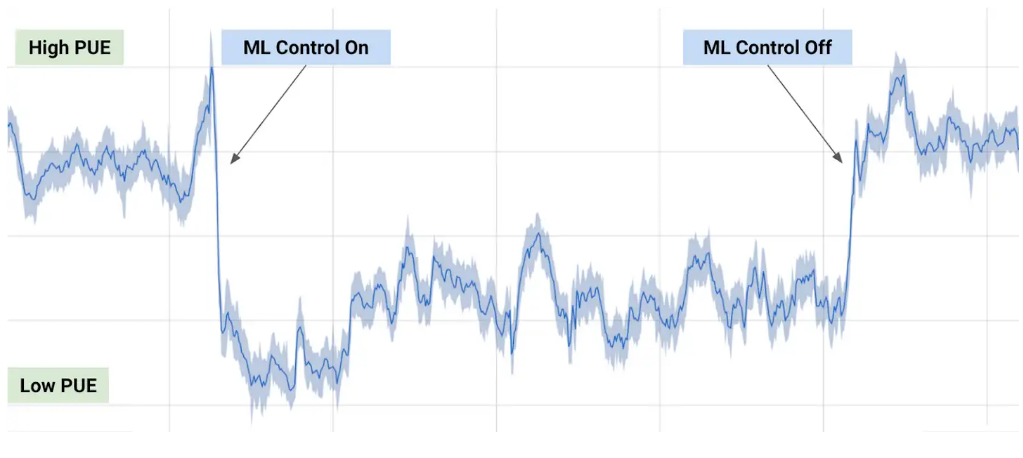
\includegraphics[width=0.7\textwidth]{images/ch5/google_data_center.jpeg}
    \caption{Power usage effectiveness with and without ML control.  Original figure from \cite{google_data1}.}
    \label{fig:google_data_center}
\end{figure}

By 2018, the agent was given full access to the data center control system after safety constraints were added. 

As a summary, the RL agents sample measurements from the sensors in each data center every five minutes and outputs the optimal control actions that satisfy a robust set of safety constraints \cite{google_data2}. The local control operators then verify the provided inputs to ensure that the system will remain within constraint boundaries. In the first few months, the agent consistently reduced electricity consumption by an average of 30\% and is expected to improve as it continues to learn. In the end, the agent reached an optimal policy that resulted in the lowest PUE ever seen, far surpassing human operation---an event only achievable through RL.
